\documentclass[a4paper, 12pt]{examen}

\begin{document}

%\modulo{Prog. multim. y de dispositivos moviles}
%\modulo{Planif. y adm. de redes}
%\modulo{Prog. de servicios y procesos}
\modulo{Lenguajes de marcas}


\pregunta{ Elabora un fichero HTML que consiga exactamente
lo que se muestra en la figura \ref{figura2}. En este ejercicio se debe escribir todo el HTML, incluyendo cabecera,
cuerpo y elementos relevante para la estructura.}{  10 }
\begin{figure}[h]
    \caption{Resultado esperable en el ejercicio 1}
    \label{figura2}
    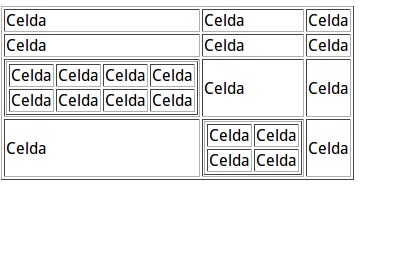
\includegraphics[scale=0.7]{foto_07.png}
\end{figure}
\break



\end{document}
